\documentclass[tikz,border=10pt]{standalone}
\usetikzlibrary{intersections}
\begin{document}
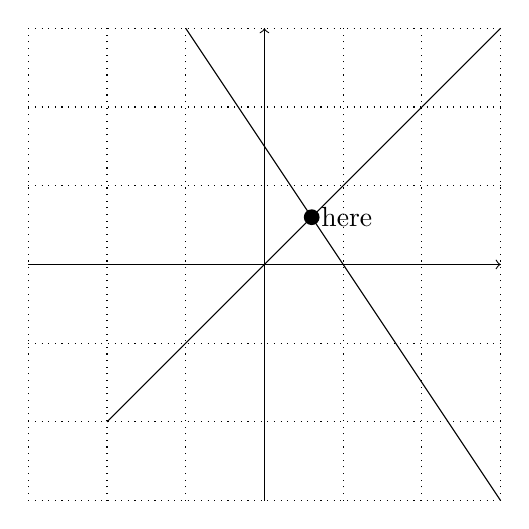
\begin{tikzpicture}
  \draw[thin,dotted] (-3,-3) grid (3,3);
  \draw[->] (-3,0) -- (3,0);
  \draw[->] (0,-3) -- (0,3);
  \draw[name path = l1] (-2,-2) -- (3,3);
  \draw[name path = l2] (-1,3)  -- (3,-3);
  \fill[name intersections = {of = l1 and l2}]
    (intersection-1) circle(1mm) node[right] {here};
\end{tikzpicture}
\end{document}
